% Taken from StackExchange at https://tex.stackexchange.com/questions/102563/how-to-draw-a-layered-architecture-using-latex
% See the answer there for a detailed explanation of the code

\documentclass{standalone}
\usepackage{tikz}
\usetikzlibrary{positioning,calc,fit}

\definecolor{mybluei}{RGB}{124,156,205}
\definecolor{myblueii}{RGB}{73,121,193}
\definecolor{mygreen}{RGB}{202,217,126}
\definecolor{mypink}{RGB}{233,198,235}

% this length is used to control the width of the light blue frame
% for the upper part of the diagram
\newlength\myframesep
\setlength\myframesep{8pt}

\pgfdeclarelayer{background}
\pgfsetlayers{background,main}

\pgfkeys{
    /tikz/node distance/.append code={
        \pgfkeyssetvalue{/tikz/node distance value}{#1}
    }
}

\newcommand\widernode[5][blueb]{
\node[
        #1,
        inner sep=0pt,
        shift=($(#2.south)-(#2.north)$),
        yshift=-\pgfkeysvalueof{/tikz/node distance value},
        fit={(#2) (#3)},
        label=center:{\sffamily\bfseries\color{white}#4}] (#5) {};
}

\begin{document}

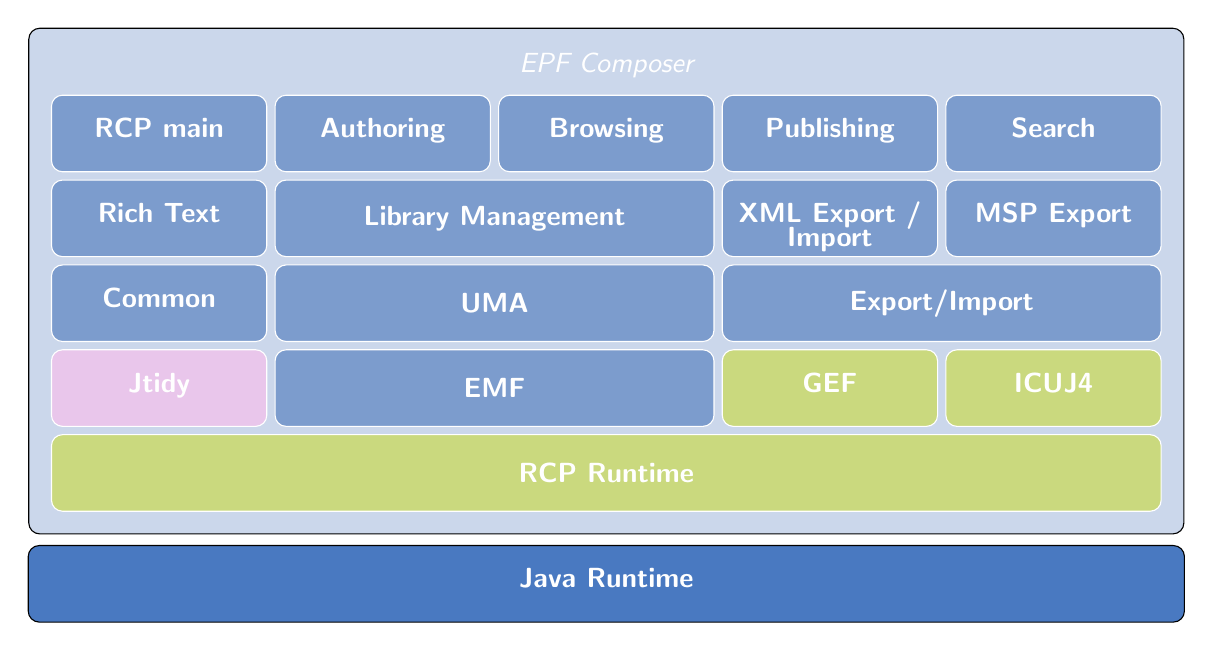
\begin{tikzpicture}[node distance=3pt,outer sep=0pt,
blueb/.style={
  draw=white,
  fill=mybluei,
  rounded corners,
  text width=2.5cm,
  font={\sffamily\bfseries\color{white}},
  align=center,
  text height=12pt,
  text depth=9pt},
greenb/.style={blueb,fill=mygreen},
]
\node[blueb] (RCP) {RCP main};
\node[blueb,right=of RCP] (Aut) {Authoring};
\node[blueb,right=of Aut] (Bro) {Browsing};
\node[blueb,right=of Bro] (Pub) {Publishing};
\node[blueb,right=of Pub] (Sea) {Search};
\node[blueb,below=of RCP] (RTe) {Rich Text};
\widernode{Aut}{Bro}{Library Management}{LMa}
\node[blueb,right=of LMa] (XML) {XML Export /\\[-0.7ex] Import};
\node[blueb,right=of XML] (MSP) {MSP Export};
\node[blueb,below=of RTe] (Com) {Common};
\widernode{LMa}{LMa}{UMA}{UMA}
\widernode{XML}{MSP}{Export/Import}{EI}
\node[blueb,fill=mypink,below=of Com] (Jti) {Jtidy};
\widernode{UMA}{UMA}{EMF}{EMF}
\node[greenb,right=of EMF] (GEF) {GEF};
\node[greenb,right=of GEF] (ICU) {ICUJ4};
\widernode[greenb]{Jti}{ICU}{RCP Runtime}{RCP}
\begin{pgfonlayer}{background}
\draw[blueb,draw=black,fill=mybluei!40]
  ([xshift=-\myframesep,yshift=3\myframesep]current bounding box.north west)
    rectangle
  ([xshift=\myframesep,yshift=-\myframesep]current bounding box.south east);
\end{pgfonlayer}
\path  let \p1=( $ (RCP.east) - (RCP.west) $ )
 in node[blueb,inner xsep=0pt,draw=black,fill=myblueii,below=4pt of current bounding box.south,text width=\x1+2*\myframesep+2\pgflinewidth] (JRu) {Java Runtime};
\node[font=\sffamily\itshape\color{white},above=of Bro] {EPF Composer};
\end{tikzpicture}

\end{document}
